%!TEX program = xelatex

\documentclass[compress]{beamer}
%--------------------------------------------------------------------------
% Common packages
%--------------------------------------------------------------------------
\usepackage[english]{babel}
\usepackage{pgfpages} % required for notes on second screen
\usepackage{graphicx}
\usepackage{subfigure}
\usepackage{multicol}
\usepackage{multirow}
\usepackage{hyperref}
\def\block(#1,#2)#3{\multicolumn{#2}{c}{\multirow{#1}{*}{$ #3 $}}}

\usepackage{fontspec}

\usepackage{tabularx,ragged2e}
\usepackage{booktabs}

\usepackage{setspace}

\usepackage{gitdags}
\usepackage[normalem]{ulem} % strikeout
%--------------------------------------------------------------------------
% Load theme
%--------------------------------------------------------------------------
\usetheme{hri}

\usepackage{tikz}
\usetikzlibrary{intersections,arrows,shapes,calc,mindmap,backgrounds,positioning,svg.path}

\graphicspath{{figs/}}

\setbeamercolor{highlightCol}{bg=hriSec3,fg=white}
\newcommand{\highlight}[1]{%
    \vspace{1em}%
    \begin{beamercolorbox}[wd=\linewidth,ht=2ex,dp=0.7ex]{highlightCol}%
    \centering #1%
    \end{beamercolorbox}%
    \vspace{1em}%
}%

\tikzset{temporal/.code args={<#1>#2#3#4}{%
          \temporal<#1>{\pgfkeysalso{#2}}{\pgfkeysalso{#3}}{\pgfkeysalso{#4}} % \pgfkeysalso doesn't change the path
}}

\newcommand{\source}[2]{{\begin{flushright}\small\it Source:\href{#1}{#2}\end{flushright}}}

%--------------------------------------------------------------------------
% General presentation settings
%--------------------------------------------------------------------------
\title{\bf software engineering 101}
\subtitle{(with a pinch of git on top)}
\date{03 Oct. 2017}
\author{Séverin Lemaignan}
\institute{Centre for Robotics \& Neural
Systems\\{\bf Plymouth University}}

%--------------------------------------------------------------------------
% Notes settings
%--------------------------------------------------------------------------
%\setbeameroption{show notes on second screen}
%\setbeameroption{hide notes}

\begin{document}

\licenseframe{https://github.com/severin-lemaignan/lecture-software-engineering/}
\maketitle





%%%%%%%%%%%%%%%%%%%%%%%%%%%%%%%%%%%%%%%%%%%%%%%%%%%%%%%%%%%%%%%%%%%%%%%%%%%%%%%
%%%%%%%%%%%%%%%%%%%%%%%%%%%%%%%%%%%%%%%%%%%%%%%%%%%%%%%%%%%%%%%%%%%%%%%%%%%%%%%
%%%%%%%%%%%%%%%%%%%%%%%%%%%%%%%%%%%%%%%%%%%%%%%%%%%%%%%%%%%%%%%%%%%%%%%%%%%%%%%
\section{Building code}

\begin{frame}{Compiled vs Not compiled}
\end{frame}

\begin{frame}[fragile]{Compiling code in C++}

\begin{cppcode}
/*
 * "Hello, World!": A classic.
 */

#include <iostream>

using namespace std;

int main(void)
{
    cout << "Hello, World!" << endl;
    return 0;
}
\end{cppcode}

\pause

\begin{shcode}
$ g++ hello.cpp -ohello
\end{shcode}

\pause 

\begin{shcode}
$ ./hello
Hello, World!
\end{shcode}

\end{frame}


\begin{frame}{Compiling code in C++: the main stages}

    \begin{enumerate}
        \item Pre-processing
        \item Compilation
        \item Assembly
        \item Linking
    \end{enumerate}

These four steps are transparently performed one after the other by your
    favourite compiler.

\end{frame}

\begin{frame}[fragile]{Compiling code in C++: Pre-processing}


\begin{cppcode}
/*
 * "Hello, World!": A classic.
 */

#include <iostream>

using namespace std;

int main(void)
{
    cout << "Hello, World!" << endl;
    return 0;
}
\end{cppcode}

Pre-processor \emph{directives} start with \cpp{#}

$\rightarrow$ \cpp{#include <iostream>} is replaced by the content of that file.

\end{frame}

\begin{frame}[fragile]{Compiling code in C++: Compilation}

\begin{shcode}
$ g++ -S hello.cpp
\end{shcode}


\begin{asmcode}
main:
.LFB1493:
	.cfi_startproc
	pushq	%rbp
	.cfi_def_cfa_offset 16
	.cfi_offset 6, -16
	movq	%rsp, %rbp
	.cfi_def_cfa_register 6
	leaq	.LC0(%rip), %rsi
	leaq	_ZSt4cout(%rip), %rdi
	call	_ZStlsISt11char_traitsIcEERSt13basic_ostreamIcT_ES5_PKc@PLT
	movq	%rax, %rdx
	movq	_ZSt4endlIcSt11char_traitsIcEERSt13basic_ostreamIT_T0_ES6_@GOTPCREL(%rip), %rax
	movq	%rax, %rsi
	movq	%rdx, %rdi
	call	_ZNSolsEPFRSoS_E@PLT
\end{asmcode}
\end{frame}

\begin{frame}[fragile]{Compiling code in C++: Assembly}

\begin{shcode}
$ g++ -s hello.cpp
$ hexdump a.out
0000000 457f 464c 0102 0001 0000 0000 0000 0000
0000010 0003 003e 0001 0000 07b0 0000 0000 0000
0000020 0040 0000 0000 0000 1128 0000 0000 0000
0000030 0000 0000 0040 0038 0009 0040 001b 001a
0000040 0006 0000 0005 0000 0040 0000 0000 0000
0000050 0040 0000 0000 0000 0040 0000 0000 0000
0000060 01f8 0000 0000 0000 01f8 0000 0000 0000
0000070 0008 0000 0000 0000 0003 0000 0004 0000
0000080 0238 0000 0000 0000 0238 0000 0000 0000
0000090 0238 0000 0000 0000 001c 0000 0000 0000
00000a0 001c 0000 0000 0000 0001 0000 0000 0000
00000b0 0001 0000 0005 0000 0000 0000 0000 0000
00000c0 0000 0000 0000 0000 0000 0000 0000 0000
00000d0 0b78 0000 0000 0000 0b78 0000 0000 0000
00000e0 0000 0020 0000 0000 0001 0000 0006 0000
...
\end{shcode}
\end{frame}

\begin{frame}[fragile]{Compiling code in C++: Linking}

The linker copies (and re-arrange) the machine code of the static dependencies
(\emph{static libraries}) into the executable.

That's what the \texttt{-l} flag is used for:

\begin{shcode}
$ g++ cool_app.cpp -ocool_app -lcv_core -lcv_highgui -lcv_videoproc
\end{shcode}

\end{frame}

\begin{frame}{Libraries}

    A library is a collection of pre-compiled functions that might get called by
    an executable. \emph{Libraries are not executable} by themselves.

    \begin{exampleblock}{Why libraries?}
        \begin{itemize}
            \item to modularise your code
            \item to make it easier to reuse
        \end{itemize}
    \end{exampleblock}

    \pause

    Two main kinds:

    \begin{itemize}
        \item Static libraries, whose code is \emph{copied} into the executable
            by the linker. Extensions: \texttt{.a}, \texttt{.lib}
        \item Dynamic libraries, whose code is \emph{loaded by the operating
            system} at runtime. They are also called \emph{shared libraries}.
            Extensions: \texttt{.so}, \texttt{.dll}, \texttt{.dylib}
    \end{itemize}

\end{frame}

\begin{frame}{Static vs Dynamic libraries}

    \only<1>{
    \begin{center}
        \Large
    Take 5 min and try to list 2 advantages for the static libraries
    on one hand, and the dynamic libraries on the other hand.
    \end{center}
    }

    \onslide<2-> {

    \textbf{Advantages of static libraries}:
    \begin{itemize}
        \item application can be certain that all its libraries are present
        \item libraries are the correct version {\small (on Linux, distributions
            and package managers handle that for dynamic libraries)}
        \item single executable: simpler distribution and installation
        \item only need to copy (and load into memory) the parts that are needed
    \end{itemize}

}
    \onslide<3->{
    \textbf{Advantages of dynamic libraries}:
    \begin{itemize}
        \item executables smaller because no need to copy the libraries' code
        \item prevent redundant code in the system
        \item allows the libraries to be easily updated to fix bugs and security flaws
            without updating each of the applications
    \end{itemize}
}
\end{frame}

\begin{frame}[fragile]{How to make \& use libraries?}

\begin{onlyenv}<1>

Code source of a pathfinding tool for our robots:

\begin{shcode}
main.cpp
ui.cpp
pathfinding.cpp
\end{shcode}

\begin{shcode}
$ g++ main.cpp ui.cpp pathfinding.cpp -opathfinding_ui
\end{shcode}


\sh{pathfinding.cpp} contains the actual pathfinder, and might be useful for
many other projects. How to turn it into a library?

\end{onlyenv}
\begin{onlyenv}<2>

First, we need to extract the \textbf{API} of our library in a
\textbf{public header} \sh{pathfinding.hpp}:

\begin{cppcode}
#ifndef _PATHFINDING_HPP
#define _PATHFINDING_HPP

class Pathfinder {

    Pathfinder(std::shared_ptr<const Map> map);
    Path find(size_t goal_x, size_t goal_y);
}

#endif
\end{cppcode}

The header contains the \textbf{declarations} of our classes, structures,
functions, but not the \textbf{definitions} (the definitions are in
\sh{pathfinding.cpp}).

\end{onlyenv}

\begin{onlyenv}<3>
Next, compile the library:

\begin{shcode}
$ g++ -fPIC -shared pathfinding.cpp -olibpathfinding.so
\end{shcode}
\end{onlyenv}

\begin{onlyenv}<4>
Finally, use it:

\begin{shcode}
$ g++ main.cpp ui.cpp -lpathfinding -opathfinding_ui
\end{shcode}
\end{onlyenv}


\end{frame}

\begin{frame}{Build system}

    Use and provide a build system!

    \begin{itemize}
        \item Windows-only $\Rightarrow$ a Visual Studio solution is ok
        \item MacOS-only $\Rightarrow$ a XCode project is ok
    \end{itemize}

    In all other cases, go for a cross-platform build system like {\bf
    CMake}.
\end{frame}

\begin{frame}[fragile]{Example of a CMake file}

%\begin{multicols}{2}
\begin{cmakecode}
cmake_minimum_required(VERSION 2.8.3)
project(cmake_example)

find_package(OpenCV REQUIRED)

include_directories(include)

add_definitions(-std=c++11)

add_executable(run src/main.cpp)
target_link_libraries(run ${OpenCV_LIBRARIES})

install(TARGETS run
   RUNTIME DESTINATION bin
)

install(FILES
    config/app.conf
    DESTINATION etc
)
\end{cmakecode}
%\end{multicols}

\end{frame}

%%%%%%%%%%%%%%%%%%%%%%%%%%%%%%%%%%%%%%%%%%%%%%%%%%%%%%%%%%%%%%%%%%%%%%%%%%%%%%%
%%%%%%%%%%%%%%%%%%%%%%%%%%%%%%%%%%%%%%%%%%%%%%%%%%%%%%%%%%%%%%%%%%%%%%%%%%%%%%%
%%%%%%%%%%%%%%%%%%%%%%%%%%%%%%%%%%%%%%%%%%%%%%%%%%%%%%%%%%%%%%%%%%%%%%%%%%%%%%%
\section{Organising your code}

\begin{frame}{}
    \centering

    \highlight{\bf principle of least surprise}

    Make people feel at home when they interact with your project!

\end{frame}

\begin{frame}[fragile]{Repository layout}

Try to follow as much as possible the {\bf Filesystem Hierarchy
 Standard} (FHS). Mainly:

\begin{shcode}
src/        # source
include/    # *public* headers
etc/        # configuration files
share/      # data
doc/        # documentation
README
LICENSE
\end{shcode}

\centering

\only<1>{
{\bf NO build artifacts!!}\\
{\bf no binaries} (except possibly in \sh{share/})
}
\only<2>{
\sh{README} (or better, use markdown: \sh{README.md}): what is
the project about? who is the target audience? how to install? how to get started?
}

\end{frame}

\begin{frame}[fragile]{Example}

\begin{onlyenv}<1>
\begin{shcode}
my_proj/
  main.cpp
  ui.cpp
  ui.hpp
  pathfinding.cpp
  pathfinding.hpp
  ui.conf
\end{shcode}

\end{onlyenv}

\begin{onlyenv}<2>
\begin{shcode}
my_proj/
  src/
    main.cpp
    ui.cpp
    ui.hpp
    pathfinding.cpp
  include/
    pathfinding.hpp
  etc/
    ui.conf
  README.md
  CMakeLists.txt
\end{shcode}

\end{onlyenv}

\begin{onlyenv}<3>
When compiling the project, create a sub-directory \sh{build} and perform an
    \textbf{out-of-tree} build:

\begin{shcode}
$ mkdir build && cd build
$ cmake ..
$ make
\end{shcode}

\end{onlyenv}

\begin{onlyenv}<4>

\begin{shcode}
build/
  ... # lots of compilation artifacts
src/
  main.cpp
  ui.cpp
  ui.hpp
  pathfinding.cpp
include/
  pathfinding.hpp
etc/
  ui.conf
README.md
CMakeLists.txt
\end{shcode}

    The \sh{build/} directory can be deleted at any point as it contains only
    generated files.
\end{onlyenv}
\end{frame}


\section{Versioning}
\begin{frame}{Semantic versioning}
    \only<1>{
    Given a version number \texttt{MAJOR.MINOR.PATCH}, increment the:

    \begin{itemize}
        \item \texttt{MAJOR} version when you make incompatible API changes,
        \item \texttt{MINOR} version when you add functionality in a backwards-compatible
manner, and
        \item \texttt{PATCH} version when you make backwards-compatible bug fixes.
    \end{itemize}

Additional labels for pre-release and build metadata are
    available as extensions to the \texttt{MAJOR.MINOR.PATCH format}.

    \source{semver.org}{\texttt{semver} website}

}

    \only<2->{

        You are the maintainer of \texttt{cool\_app}, that depends on OpenCV
        \texttt{2.4.11}.

        The OpenCV project releases a new version, what should you do...

        \begin{itemize}
            \item <2-> ...if the new version is \texttt{2.4.12}?
            \item <3-> ...if the new version is \texttt{2.5.0}?
            \item <4-> ...if the new version is \texttt{2.9.0}?
            \item <5-> ...if the new version is \texttt{3.0.0-beta}?
            \item <6-> ...if the new version is \texttt{3.0.0}?
        \end{itemize}
    }
\end{frame}


%%%%%%%%%%%%%%%%%%%%%%%%%%%%%%%%%%%%%%%%%%%%%%%%%%%%%%%%%%%%%%%%%%%%%%%%%%%%%%%
%%%%%%%%%%%%%%%%%%%%%%%%%%%%%%%%%%%%%%%%%%%%%%%%%%%%%%%%%%%%%%%%%%%%%%%%%%%%%%%
%%%%%%%%%%%%%%%%%%%%%%%%%%%%%%%%%%%%%%%%%%%%%%%%%%%%%%%%%%%%%%%%%%%%%%%%%%%%%%%
\section{Softawre Licenses, Open-source, free software}

\begin{frame}{Software licenses}
    \begin{itemize}
        \item<+-> {\bf no license} $\Rightarrow$ default copyright laws apply.
            You retain all rights to your source code; nobody else may
            reproduce, distribute, or create derivative works from your work.
        \item<+-> {\bf Permissive licenses}: others do essentially whatever they
            want with your code, as long as they give your attribution.
            Examples: MIT, BSD
        \item<+-> {\bf Copyleft licenses}: Derivative work must be made
            available under the same terms as the original work (\emph{viral
            licenses}). Example: GPL
    \end{itemize}

    \only<1-3>{
    \begin{center}
        \includegraphics[width=0.2\paperheight]{osi}\hspace{1em}
        
\includegraphics[width=0.2\paperheight]{GPLv3}
    \end{center}
    }

    \centering
    \only<4>{
        {\bf You always keep the author rights!}\\
        $\Rightarrow$ you can change the
        license at any time.
    }

    \only<5>{
    Check \url{http://choosealicense.com/}
    }


\end{frame}

\begin{frame}{What if you want to use a GPL library?}
    There is a legal dispute to know whether merely \emph{linking} with a
    library result in a \emph{derivative work} (which would then have to be
    licensed as GPL).

    \pause

    The LGPL (\emph{Lesser GPL}) explicitely allows the usage of the library
    without putting restrictions on the licensing of the resulting executable.

\end{frame}

\begin{frame}{}

    \begin{exampleblock}{Open-source vs Free software?}
    ``When we call software "free," we mean that it respects the users' essential
    freedoms: the freedom to run it, to study and change it, and to redistribute
    copies with or without changes. This is a matter of freedom, not price, so
    think of "free speech," not "free beer."''

        \vspace{1em}
    ``Open source is a development methodology; free software is a social
        movement''

    \end{exampleblock}

    \source{https://www.gnu.org/philosophy/open-source-misses-the-point.en.html}{GNU
    website}
\end{frame}

%%%%%%%%%%%%%%%%%%%%%%%%%%%%%%%%%%%%%%%%%%%%%%%%%%%%%%%%%%%%%%%%%%%%%%%%%%%%%%%
%%%%%%%%%%%%%%%%%%%%%%%%%%%%%%%%%%%%%%%%%%%%%%%%%%%%%%%%%%%%%%%%%%%%%%%%%%%%%%%
%%%%%%%%%%%%%%%%%%%%%%%%%%%%%%%%%%%%%%%%%%%%%%%%%%%%%%%%%%%%%%%%%%%%%%%%%%%%%%%

\section{Git}

\imageframe[color=black, scale=0.95]{first_mention_git}
\imageframe[color=black, scale=0.95]{windows_on_git_announcement}

\imageframe[color=black, caption=These directories are git repositories]{windows-explorer/explorer-base}
\imageframe[color=black, caption=They look boringly normal]{windows-explorer/explorer-gitrepo}

\begin{frame}[plain]
    A few roundtrips later with colleagues...
\end{frame}

\imageframe{zipfiles}
\imageframe{dropbox_zipfiles}
\imageframe{dropbox_zipfiles_devil}

{
    \fullbackground{../figs/facebook-wall.png}
    \begin{frame}[plain]{}
        \only<2>{
            \begin{center}
                
\includegraphics[width=\linewidth]{devil}
            \end{center}
        }
    \end{frame}
}


\begin{frame}{}
    \begin{center}
        \textbf{We can do better!}
    \end{center}
    \pause

    \textbf{git} is essentially about recording the history of files
    \pause

    (and who did what)
    \pause

    (and sharing as well)
\end{frame}

\section{Versioning}

\begin{frame}{Why versioning?}

    \begin{itemize}
        \item The history of your development/document
        \item Compare the current code with an older version
        \item Roll-back to previous versions
        \item Experiment without losing anything
        \item Trace who did what (at the level of the line of code)
        \item Annotate your workflow (important milestones, etc)
        \item Avoid catastrophes!
    \end{itemize}
\end{frame}

\begin{frame}{Atomic commits}

    The single most important concept (because it requires to think about
    development/writing in terms of {\bf functional units}):

    \highlight{Atomic commit}

    \only<1>{
        A (typically small) commit that represent a {\bf single, coherent \&
    complete} functional change.
    }
    \only<2>{
    \begin{itemize}
        \item Easy to understand the change
        \item Debugging made easy (\texttt{git bisect})
        \item Collaboration made easy (less, smaller conflict)
        \item Easy to write a useful commit message
    \end{itemize}
    }

\end{frame}

\begin{frame}[fragile]{}

\centering

\begin{tikzpicture}[
    >=latex,
    every edge/.style={draw,thick,hriSec3},
    file/.style={align=left, inner sep=1pt,font=\scriptsize\tt}
]

\node at (-2, 1.5)[file,temporal=<4>{red}{black}{white}] (file1) {\sout{main.cpp}};
\node [file,temporal=<4>{red}{black}{white},below=0.0 of file1.south east,anchor=north east] (file2) {src/main.cpp};
\node [file,temporal=<2>{red}{black}{white},below=0.0 of file2.south east, anchor=north east] (file3) {src/position.cpp};
\node [file,temporal=<2>{red}{black}{white},below=0.0 of file3.south east,anchor=north east] (file4) {src/position.hpp};
\node [file,temporal=<3>{red}{black}{white},below=0.0 of file4.south east,anchor=north east] (file5) {share/model.csv};


    \onslide<2>{
        \gitDAG[grow right sep = 2em]{
            A;
        };

        \gitbranch
        {master}
        {above=of A}
        {A}

        \gitHEAD
        {above=of master}
        {master}


    \path[draw] (file3.east) edge [->, bend left] (A);
    \path[draw] (file4.east) edge [->, bend left] (A);

    }
    \onslide<3>{
        \gitDAG[grow right sep = 2em]{
            A -- B;
        };

        \gitbranch
        {master}
        {above=of B}
        {B}

        \gitHEAD
        {above=of master}
        {master}

        \path[draw] (file5.east) edge [->, bend left,hriSec2] (B);
    }

    \onslide<4->{
        \gitDAG[grow right sep = 2em]{
            A -- B -- C;
        };

        \gitbranch
        {master}     % node name and text 
        {above=of C} % node placement
        {C}          % target

        \gitHEAD
        {above=of master} % node placement
        {master}          % target

        \path[draw] (file1.east) edge [->, bend left,hriSec1Comp] (C);
        \path[draw] (file2.east) edge [->, bend left,hriSec1Comp] (C);
    }

\end{tikzpicture}

\vspace{3em}
\small
\only<2>{
\texttt{git add src/position.*}\\
\texttt{git commit -m"Fix computation of position (float->double)"}
}
\only<3>{
\texttt{git add share/model.csv}\\
\texttt{git commit -m"Re-trained model with 52 more participants"}
}
\uncover<4>{
\texttt{git rm main.cpp}\\
\texttt{git add src/main.cpp}\\
\texttt{git commit -m"Move main.cpp to src/"}
}

\end{frame}

\begin{frame}[fragile]{Log}
\begin{shcode}
$ git log
commit fa009cd7fca05b0b61170b20cf76a5f72b8843c2
Author: Severin Lemaignan <severin.lemaignan@plymouth.ac.uk>
Date:   Wed Feb 10 16:48:22 2016 +0000

    Move main.cpp to src/

commit aff81119459d9193c09effef1c150c4f7eac08dc
Author: Severin Lemaignan <severin.lemaignan@plymouth.ac.uk>
Date:   Wed Feb 10 16:48:02 2016 +0000

    Re-trained model with 52 more participants

commit 4113b9b6e6bbc8de532ad90153e0059cb5819de7
Author: Severin Lemaignan <severin.lemaignan@plymouth.ac.uk>
Date:   Wed Feb 10 16:47:46 2016 +0000

    Fix computation of position (float->double)
\end{shcode}


\end{frame}

\begin{frame}{}

\centering

\begin{tikzpicture}
        \gitDAG[grow right sep = 2em]{
            4113b9 -- aff811 -- fa009c;
        };

        \gitbranch
        {master}     % node name and text 
        {above=of fa009c} % node placement
        {fa009c}          % target

        \gitHEAD
        {above=of master} % node placement
        {master}          % target

\end{tikzpicture}

\end{frame}

\begin{frame}{The staging area}
    \centering
    \only<1>{
        But why do we have to manually tell Git what files to add or remove?
    }
    \only<2>{
        No ``commit all changes'' by default {\tiny (well, you
        can, actually...)}\\
        $\Rightarrow$ Help thinking in terms of atomic commits!
    }
    \only<3->{
        Preparing a commit consists in filling the {\bf staging area} (or
        {\bf index}) with the list of changes:

        \begin{tikzpicture}[
                >=latex,
                every edge/.style={draw,thick,hriSec3},
                file/.style={align=left, inner sep=1pt,font=\scriptsize\tt}
            ]

            \node at (-3.5, 2)[file,red] (file1) {\sout{main.cpp}};
            \node [file,red,below=0.0 of file1.south east,anchor=north east] (file2) {src/main.cpp};
            \node [file,temporal=<3>{red}{black}{white},below=0.0 of file2.south east, anchor=north east] (file3) {src/position.cpp};
            \node [file,temporal=<3>{red}{black}{white},below=0.0 of file3.south east,anchor=north east] (file4) {src/position.hpp};
            \node [file,red,below=0.0 of file4.south east,anchor=north east] (file5) {share/model.csv};


            \node[gitSA,] (stagingarea) at (-2.5,3) {staging area};

            \onslide<3>{
                \gitDAG[grow right sep = 2em]{
                    154ce2 -- f327ba;
                };

                \gitbranch
                {master}     % node name and text 
                {above=of f327ba} % node placement
                {f327ba}          % target

                \gitHEAD
                {above=of master} % node placement
                {master}          % target



                \path[draw] (file3.east) edge [->, bend right,hriSec1Comp] (stagingarea);
                \path[draw] (file4.east) edge [->, bend right,hriSec1Comp] (stagingarea);

            }
            \onslide<4>{
                \gitDAG[grow right sep = 2em]{
                    154ce2 -- f327ba -- 4113b9;
                };

                \gitbranch
                {master}     % node name and text 
                {above=of 4113b9} % node placement
                {4113b9}          % target

                \gitHEAD
                {above=of master} % node placement
                {master}          % target

                \node[highlighted commit] at (4113b9) {\phantom{4113b9}};
                \draw[resetarrows] ([xshift=-1em,yshift=-1em]stagingarea.east) to[bend
                left] (4113b9.north west);

            }



        \end{tikzpicture}


        \only<3>{
            \texttt{git add}\\
            \texttt{git rm}\\
            \texttt{git add -p}\\
            ...\\
        }
        \only<4>{
            ~\\
            \texttt{git commit}\\
            ~\\
            ~\\
        }


    }
\end{frame}

\begin{frame}[fragile]{To summarize...}

The first time...
\begin{shcode}
$ mkdir my_repo && cd my_repo
$ git init
\end{shcode}
Then...
\begin{shcode}
# make some changes...
$ git add <files>
$ git commit -m"<commit message>"
# make some changes...
$ git add <files>
$ git commit -m"<other commit message>"
# That's it!
\end{shcode}


\end{frame}


\begin{frame}{}
    \centering
    Viewed from a GUI (macOS \& Windows)\\
    {\bf GitHub Desktop} Walkthrough\par
    \vspace{3em}
    \url{https://desktop.github.com/}
\end{frame}

\imageframe[caption=Log in to your GitHub account,color=black]{github-windows/1}
\imageframe[caption=Create a (local) repository,color=black]{github-windows/2}
\imageframe[caption=GitHub Desktop has already made a first commit on your behalf,color=black]{github-windows/3}
\imageframe[caption=Open the repo in Windows Explorer,color=black]{github-windows/4}
\imageframe[caption=Add a simple README.md...,color=black]{github-windows/5}
\imageframe[caption=The change is listed in the Changes panel,color=black]{github-windows/6}
\imageframe[caption=Write a commit message \& commit!,color=black]{github-windows/7}
\imageframe[caption=The History panel shows the log and a diff of your changes,color=black]{github-windows/8}

\begin{frame}{}
    Viewed from a GUI\\
    {\bf Tortoise GIT}\par
    \vspace{3em}
    \url{https://tortoisegit.org/}
\end{frame}

\imageframe[color=black,caption=Direct interaction in the Windows explorer]{tortoise-git/gitcommit}
\imageframe[color=black,caption=Files' status appear as icons]{tortoise-git/overlays}
\imageframe[color=black,caption=All the functionalities are available]{tortoise-git/contextmenu}
\imageframe[color=black,caption=Commit window]{tortoise-git/commit}

\begin{frame}{What should be tracked?}

    Short answer: \textbf{everything you care about in your project}
    \pause

    (you can left out temporary files, automatically generated files, etc)
    \pause

    However, versioning is \textbf{less useful for binary files}: 

    \begin{itemize}
        \item no line-by-line tracking of changes
        \item every single change creates a whole copy: repo size might grow
            quickly!
    \end{itemize}

    Binary files include images, archives (zip files), \textbf{PDF},
    \textbf{most office document (docx/xlsx/pptx)}
    \pause

    For documents, you might want to consider alternative like
    \href{https://en.wikipedia.org/wiki/Markdown\#Example}{markdown}.

\end{frame}

\imageframe[color=black, caption=What should I track here?]{windows-explorer/explorer-gitrepo}

\section{Collaborating}

\imageframe{dvcs-1}
\imageframe{dvcs-2}
\imageframe{dvcs-3}
\imageframe{dvcs-4}
\imageframe{dvcs-5}
\imageframe{dvcs-6}
\imageframe{dvcs-7}
\imageframe{dvcs-8}



\begin{frame}[fragile]{}

\centering

    \begin{tikzpicture}
    % Commit DAG
    \onslide<1-3>{
      \gitDAG[grow right sep = 2em]{
        A -- B -- C;
      };

      % Branch
      \gitbranch
        {master}     % node name and text 
        {above=of C} % node placement
        {C}          % target
    }



      % HEAD reference
    \onslide<1-2>{
      \gitHEAD
        {above=of master} % node placement
        {master}          % target
    }

    \onslide<3>{
      \gitremotebranch
        [origmaster]    % node name
        {origin/master} % node text
        {above=of master}    % node placement
        {master}             % target
      \gitHEAD
        {above=of origmaster} % node placement
        {origmaster}          % target
    }

    \end{tikzpicture}

\vspace{3em}
    \begin{overlayarea}{\textwidth}{5cm}
\only<2>{
\small
\texttt{git remote add origin git@github.com:user/repo.git}\par
\scriptsize
\texttt{git remote add john-usb E:\textbackslash john\_repo}\\
\texttt{git remote add ftp-origin ftp://host.xz/path/to/repo.git/}\\
...\\
}

\only<3>{
\Large
\texttt{git push origin master} \par
\normalsize
(or simply \texttt{git push})
}
\end{overlayarea}
\end{frame}

\begin{frame}[fragile]{}

    \centering

    \begin{tikzpicture}
        \onslide<1-2>{
            \gitDAG[grow right sep = 2em]{
                A -- B -- C -- D -- E;
            };

            % Branch
            \gitbranch
            {master}     % node name and text 
            {above=of E} % node placement
            {E}          % target

            % HEAD reference
            \gitHEAD
            {above=of master} % node placement
            {master}          % target

            \gitremotebranch
            [origmaster]    % node name
            {origin/master} % node text
            {above=of C}    % node placement
            {C}             % target
        }

        \onslide<3>{
            \gitDAG[grow right sep = 2em]{
                A -- B -- C -- {
                    F,
                    D -- E,
                }
            };

            % Branch
            \gitbranch
            {master}     % node name and text 
            {above=of E} % node placement
            {E}          % target

            % HEAD reference
            \gitHEAD
            {above=of master} % node placement
            {master}          % target

            \gitremotebranch
            [origmaster]    % node name
            {origin/master} % node text
            {above=of F}    % node placement
            {F}             % target
        }

        \onslide<4-5>{
            \gitDAG[grow right sep = 2em]{
                A -- B -- C -- {
                    F -- D' -- E',
                    {[nodes=unreachable] D -- E },
                }
            };

            % Branch
            \gitbranch
            {master}     % node name and text 
            {above=of E'} % node placement
            {E'}          % target

            % HEAD reference
            \gitHEAD
            {above=of master} % node placement
            {master}          % target

            \gitremotebranch
            [origmaster]    % node name
            {origin/master} % node text
            {above=of F}    % node placement
            {F}             % target
        }

        \onslide<6->{
            \gitDAG[grow right sep = 2em]{
                A -- B -- C -- {
                    F -- D' -- E',
                    {[nodes=unreachable] D -- E },
                }
            };

            % Branch
            \gitbranch
            {master}     % node name and text 
            {above=of E'} % node placement
            {E'}          % target


            \gitremotebranch
            [origmaster]    % node name
            {origin/master} % node text
            {above=of master}    % node placement
            {master}             % target

            \gitHEAD
            {above=of origmaster} % node placement
            {origmaster}          % target
        }


    \end{tikzpicture}

    \vspace{3em}
    \begin{overlayarea}{\textwidth}{5cm}
    \only<2>{
        What happened on our remote? Let's have a look...\\
        \Large
        \texttt{git fetch origin}\\
    }

    \only<4>{
        \Large
        \texttt{git rebase origin/master}\par
        \normalsize
        (but you don't need it, because...)\\
    }
    \only<5>{
        \Large
        \texttt{git pull --rebase}\\
    }
    \only<6>{
        \Large
        \texttt{git push}\\
    }
    \end{overlayarea}

\end{frame}



\begin{frame}[fragile]{To summarize...}

The first time...
\begin{shcode}
$ git clone <url>
# for instance,
# git clone https://github.com/user/repo.git
\end{shcode}
Then...
\begin{shcode}
$ cd <repo>
# make some changes...
$ git add <files>
$ git commit -m"<commit message>"
# ...
# when you want to share:
$ git pull --rebase # any changes on the remote?
$ git push
\end{shcode}

\end{frame}

\section{The dreadful conflicts}

\begin{frame}[fragile]{The dreadful conflict}

    While peacefully editing your last (great) paper...

\begin{shcode}
$ git pull --rebase john master
First, rewinding head to replay your work on top of it...
Applying: Better terminology
Using index info to reconstruct a base tree...
M	main.tex
Falling back to patching base and 3-way merge...
Auto-merging main.tex
CONFLICT (content): Merge conflict in main.tex
error: Failed to merge in the changes.
Patch failed at 0001 Better terminology
The copy of the patch that failed is found in: .git/rebase-apply/patch

When you have resolved this problem, run "git rebase --continue".
If you prefer to skip this patch, run "git rebase --skip" instead.
To check out the original branch and stop rebasing, run "git rebase --abort".
\end{shcode}
\end{frame}

\begin{frame}[fragile]{}
\begin{shcode}
$ git pull --rebase john master
# conflict!
$ git mergetool
\end{shcode}
\end{frame}

\imageframe[color=black,caption=Meld is one of the nice tools to fix conflicts]{meld}

\section{Social coding: GitHub workflow}

\imageframe[caption=GitHub,color=black]{github-morse}
\imageframe[caption=BitBucket,color=black]{bitbucket}
\imageframe[caption=GitLab -- open-source You can install it on your own server,color=black]{gitlab}

\imageframe[color=black]{github-morse}

\imageframe{github-workflow-1}
\imageframe{github-workflow-2}
\imageframe{github-workflow-3}
\imageframe{github-workflow-4}
\imageframe{github-workflow-5}
\imageframe{github-workflow-6}


\begin{frame}[fragile]{What happened exactly?}

    \vspace{1em}
    \centering

    \begin{multicols}{2}
        \resizebox{\columnwidth}{!}{%
    \begin{tikzpicture}
        \onslide<1>{
            \gitDAG[grow right sep = 2em]{
                A -- B -- C -- D -- E;
            };

            % Branch
            \gitbranch
            {master}     % node name and text 
            {above=of E} % node placement
            {E}          % target

            % HEAD reference
            \gitHEAD
            {above=of master} % node placement
            {master}          % target

            \gitremotebranch
            [origmaster]    % node name
            {origin/master} % node text
            {above=of C}    % node placement
            {C}             % target
        }

        \onslide<2>{
            \gitDAG[grow right sep = 2em]{
                A -- B -- C -- {
                    F,
                    D -- E,
                }
            };

            % Branch
            \gitbranch
            {master}     % node name and text 
            {above=of E} % node placement
            {E}          % target

            \gitremotebranch
            [johnmaster]    % node name
            {john/master} % node text
            {above=1.2 of F}    % node placement
            {F}             % target


            \gitremotebranch
            [origmaster]    % node name
            {origin/master} % node text
            {above=of C}    % node placement
            {C}             % target

            \gitHEAD
            {above=of master} % node placement
            {master}          % target

        }

        \onslide<3>{
            \gitDAG[grow right sep = 2em]{
                A -- B -- C -- {
                    F -- D' -- E',
                    {[nodes=unreachable] D -- E },
                }
            };

            % Branch
            \gitbranch
            {master}     % node name and text 
            {above=of E'} % node placement
            {E'}          % target

            \gitremotebranch
            [origmaster]    % node name
            {origin/master} % node text
            {above=of C}    % node placement
            {C}             % target

            \gitremotebranch
            [johnmaster]    % node name
            {john/master} % node text
            {above=1.2 of F}    % node placement
            {F}             % target


            \gitHEAD
            {above=of master} % node placement
            {master}          % target


        }
        \onslide<4>{
            \gitDAG[grow right sep = 2em]{
                A -- B -- C -- {
                    F -- D' -- E',
                    {[nodes=unreachable] D -- E },
                }
            };

            % Branch
            \gitbranch
            {master}     % node name and text 
            {above=of E'} % node placement
            {E'}          % target

            \gitremotebranch
            [origmaster]    % node name
            {origin/master} % node text
            {above=of master}    % node placement
            {master}             % target

            \gitremotebranch
            [johnmaster]    % node name
            {john/master} % node text
            {above=1.2 of F}    % node placement
            {F}             % target


            \gitHEAD
            {above=of origmaster} % node placement
            {origmaster}          % target


        }

    \end{tikzpicture}
    }

    \only<1>{
        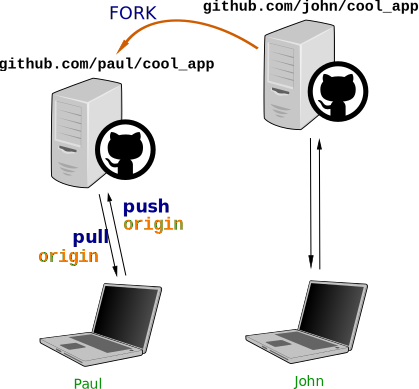
\includegraphics[width=0.8\columnwidth]{github-workflow-details-3}
    }
    \only<2-3>{
        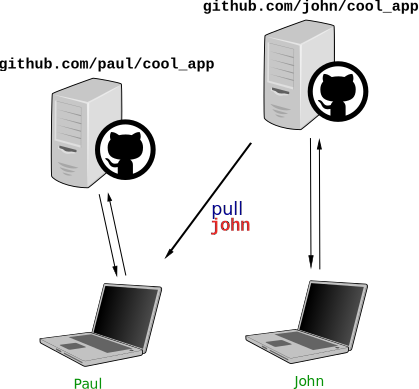
\includegraphics[width=0.8\columnwidth]{github-workflow-details-5}
    }

    \only<4>{
        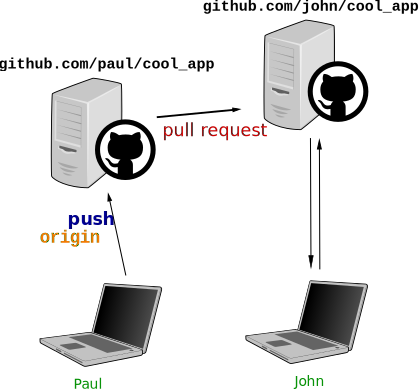
\includegraphics[width=0.8\columnwidth]{github-workflow-details-6}
    }

    \end{multicols}

    \begin{overlayarea}{\textwidth}{5cm}
    \only<1>{
        After forking on GitHub, Paul runs\\
        \texttt{git clone https://github.com/paul/cool\_app.git}\\
        \normalsize
        and he adds few local commits\\
    }

    \only<2>{
        He would like to propose his changes to John\\
        First, he needs to get the latest changes from John:\par
        \footnotesize
        \texttt{git add remote john https://github.com/john/cool\_app.git}\\
        \normalsize
        \texttt{git fetch john}\\
    }

    \only<3>{
        Paul rebases his \texttt{master} branch on John's one:\par
        \texttt{git rebase john/master}\par
        \footnotesize
        (actually, Paul would simply run \texttt{git pull --rebase john master})
    }
    \only<4>{
        He pushes his commits to his own GitHub account:\par
        \texttt{git push}\\
        ...and finally press the ``Create a pull request'' button in GitHub.
    }

\end{overlayarea}
\end{frame}

\begin{frame}{}
    \centering
    (what happens next on John's side is a story for another day :-) But to make
    it short, he can press ``Merge pull request'' on his GitHub account if he is
    happy with the pull-request!)
\end{frame}
\imageframe{github-workflow-7}


\section{The one slide to remember}

\begin{frame}{GIT cheat sheet}
\scriptsize
    \begin{multicols}{2}

    {\bf To start...}\\
    ...from scratch: \texttt{git init}\\
    ...from existing repo: \texttt{git clone <url>}\par

    \rule{\columnwidth}{0.2pt}

    {\bf Prepare commits:}\\
    \texttt{git add}\\
    \texttt{git rm}\\
    \texttt{git add -p} (partial files)\par

    {\bf Commit:}\\
    \texttt{git commit}\par

    \rule{\columnwidth}{0.2pt}

    {\bf Create branch:}\\
    \texttt{git checkout -b <branch>}\par

    {\bf Jump between branches:}\\
    \texttt{git checkout <branch>}\par

    {\bf ``Import'' another branch:}\\
    \texttt{git rebase <other\_branch>}\par

    \rule{\columnwidth}{0.2pt}

    {\bf Add a remote source:}\\
    \texttt{git remote add <name> <url>}\par

    {\bf What's new on a remote?}\\
    \texttt{git pull <remote> <branch>}\\
    {\tiny (\texttt{git pull} alone $\equiv$ \texttt{git pull origin master})}\par

    {\bf Share stuff on a remote:}\\
    \texttt{git push <remote> <branch>}\\
    {\tiny (\texttt{git push} alone $\equiv$ \texttt{git push origin master})}\par

    \rule{\columnwidth}{0.2pt}

    \begin{multicols}{2}
    {\bf Repo state}\\
    \texttt{git status}\par

    {\bf Repo history}\\
    \texttt{git log}\par

    {\bf Who did what?}\\
    \texttt{git blame}\par

    {\bf I've lost everythg!}\\
    \texttt{git reflog}\par


    \end{multicols}

    ~\\

    \end{multicols}

\end{frame}

{
    \fullbackground{background}
\begin{frame}[plain]
        \Large
        That's all, folks!\\[2em]
        \normalsize
        Questions:\\
        Portland Square B316 or \url{severin.lemaignan@plymouth.ac.uk} \\[1em]

        Slides:
        \href{https://github.com/severin-lemaignan/lecture-software-engineering}{\small
        github.com/severin-lemaignan/lecture-software-engineering}

\end{frame}
}

\appendix

\begin{frame}{Supplementary material}
    \tableofcontents[hideallsubsections]
    %\tableofcontents
\end{frame}


\section{Working with branches}

\begin{frame}{Branches}

    \centering

    \begin{tikzpicture}
        \only<1-5>{
        \onslide<1>{
            \gitDAG[grow right sep = 2em]{
                A -- B -- C;
            };

            % Branch
            \gitbranch
            {master}     % node name and text 
            {above=of C} % node placement
            {C}          % target

            % HEAD reference
            \gitHEAD
            {above=of master} % node placement
            {master}          % target

        }

        \onslide<2>{
            \gitDAG[grow right sep = 2em]{
                A -- B -- C;
            };

            % Branch
            \gitbranch
            {master}     % node name and text 
            {above=of C} % node placement
            {C}          % target

            \gitbranch
            {cool-idea}     % node name and text 
            {above=of master} % node placement
            {master}          % target

            % HEAD reference
            \gitHEAD
            {above=of cool-idea} % node placement
            {cool-idea}          % target
        }

        \onslide<3>{
            \gitDAG[grow right sep = 2em]{
                A -- B -- C -- D -- E;
            };

            % Branch
            \gitbranch
            {master}     % node name and text 
            {above=of C} % node placement
            {C}          % target

            \gitbranch
            {cool-idea}     % node name and text 
            {above=of E} % node placement
            {E}          % target

            % HEAD reference
            \gitHEAD
            {above=of cool-idea} % node placement
            {cool-idea}          % target
        }

        \onslide<4>{
            \gitDAG[grow right sep = 2em]{
                A -- B -- C -- D -- E;
            };

            % Branch
            \gitbranch
            {master}     % node name and text 
            {above=of C} % node placement
            {C}          % target

            \gitbranch
            {cool-idea}     % node name and text 
            {above=of E} % node placement
            {E}          % target

            % HEAD reference
            \gitHEAD
            {above=of master} % node placement
            {master}          % target
        }

        \onslide<5>{
            \gitDAG[grow right sep = 2em]{
                A -- B -- C -- {
                    D -- E,
                    F -- G -- H,
                }
            };

            % Branch
            \gitbranch
            {master}     % node name and text 
            {above=of H} % node placement
            {H}          % target

            \gitbranch
            {cool-idea}     % node name and text 
            {above=of E} % node placement
            {E}          % target

            % HEAD reference
            \gitHEAD
            {above=of master} % node placement
            {master}          % target
        }
    }
        \only<6->{
            \gitDAG[grow right sep = 1.5em]{
                A -- B -- C -- {
                    D -- E,
                    F -- G -- H -- {
                        K,
                        I -- J
                        },
                }
            };

            % Branch
            \gitbranch
            {master}     % node name and text 
            {above=of K} % node placement
            {K}          % target

            \gitbranch
            {cool-idea}     % node name and text 
            {above=of E} % node placement
            {E}          % target

            \gitbranch
            {bug142}     % node name and text 
            {above=of J} % node placement
            {J}          % target


            % HEAD reference
            \gitHEAD
            {above=of master} % node placement
            {master}          % target
        }


    \end{tikzpicture}

    \vspace{3em}
    \centering
    \only<1>{
        What if...?\\
    }
    \only<2>{
        \Large
        \texttt{git checkout -b cool-idea}\\
    }
    \only<5>{
        The branch name is an alias for the tip of the current branch\\
    }
    \only<6>{
        $\Rightarrow$ branches are very cheap\\ 
        +10 of them at a given time it not uncommon\\
    }
    \uncover<4>{
        Let go back to serious stuff!\\
        \Large
        \texttt{git checkout master}
    }


\end{frame}


\begin{frame}{Merging branches}

    \centering

\begin{tikzpicture}[
    >=latex,
    every edge/.style={draw,thick,hriSec3}
]

        \onslide<1>{
            \gitDAG[grow right sep = 2em]{
                B -- C -- {
                    D -- E,
                    F -- G -- H,
                };
            };

            % Branch
            \gitbranch
            {master}     % node name and text 
            {above=of H} % node placement
            {H}          % target

            \gitbranch
            {cool-idea}     % node name and text 
            {above=of E} % node placement
            {E}          % target

            % HEAD reference
            \gitHEAD
            {above=of master} % node placement
            {master}          % target

            \node[DAGcommit,right=3 of E.south,dashed] (merge) {?};
            \path[draw] (E) edge [->, bend left] (merge);
            \path[draw] (H) edge [->, bend right] (merge);
    }
        \onslide<2>{
            \gitDAG[grow right sep = 2em]{
                B -- C -- {
                    D -- E,
                    F -- G -- H -- merge,
                };

                E -- merge;
            };

            % Branch
            \gitbranch
            {master}     % node name and text 
            {above=of merge} % node placement
            {merge}          % target

            \gitbranch
            {cool-idea}     % node name and text 
            {above=of E} % node placement
            {E}          % target

            % HEAD reference
            \gitHEAD
            {above=of master} % node placement
            {master}          % target

    }
        \onslide<3>{
            \gitDAG[grow right sep = 2em]{
                B -- C -- {
                    D -- E,
                    F -- G -- H -- I -- J,
                };

                E -- I;
            };

            % Branch
            \gitbranch
            {master}     % node name and text 
            {above=of J} % node placement
            {J}          % target

            \gitbranch
            {cool-idea}     % node name and text 
            {above=of E} % node placement
            {E}          % target

            % HEAD reference
            \gitHEAD
            {above=of master} % node placement
            {master}          % target

    }
        \onslide<4>{
            \gitDAG[grow right sep = 2em]{
                B -- C -- {
                    D -- E -- K -- L,
                    F -- G -- H -- I -- J,
                };

                E -- I;
            };

            % Branch
            \gitbranch
            {master}     % node name and text 
            {above=of J} % node placement
            {J}          % target

            \gitbranch
            {cool-idea}     % node name and text 
            {above=of L} % node placement
            {L}          % target

            % HEAD reference
            \gitHEAD
            {above=of cool-idea} % node placement
            {cool-idea}          % target

    }



    \end{tikzpicture}

    \vspace{3em}
    \centering
    \only<1>{
        Two options: {\bf merging} and {\bf rebasing}\\
    }
    \only<2>{
        Merging\\
        \Large
        \texttt{git merge cool-idea}\\
    }
    \only<3>{
        \Large
        \texttt{git commit}\\
    }
    \uncover<4>{
        \Large
        \texttt{git checkout cool-idea}\\
        \texttt{git commit}\\
        \normalsize
        ...etc.
    }


\end{frame}

\begin{frame}{Rebasing branches}

    \centering

\begin{tikzpicture}[
    >=latex,
    every edge/.style={draw,thick,hriSec3}
]

        \onslide<1>{
            \gitDAG[grow right sep = 2em]{
                B -- C -- {
                    D -- E,
                    F -- G -- H,
                };
            };

            % Branch
            \gitbranch
            {master}     % node name and text 
            {above=of H} % node placement
            {H}          % target

            \gitbranch
            {cool-idea}     % node name and text 
            {above=of E} % node placement
            {E}          % target

            % HEAD reference
            \gitHEAD
            {above=of master} % node placement
            {master}          % target

            \node[DAGcommit,right=3 of E.south,dashed] (merge) {?};
            \path[draw] (E) edge [->, bend left] (merge);
            \path[draw] (H) edge [->, bend right] (merge);
    }
        \onslide<2>{
            \gitDAG[grow right sep = 2em]{
                B -- C -- {
                    D -- E -- F' -- G' -- H',
                    {[nodes=unreachable] F -- G -- H },
                };
            };

            % Branch
            \gitbranch
            {master}     % node name and text 
            {above=of H'} % node placement
            {H'}          % target

            \gitbranch
            {cool-idea}     % node name and text 
            {above=of E} % node placement
            {E}          % target

            % HEAD reference
            \gitHEAD
            {above=of master} % node placement
            {master}          % target

    }
        \onslide<3>{
            \gitDAG[grow right sep = 2em]{
                B -- C -- {
                    D -- E -- {
                        I -- J,
                        F' -- G' -- H',
                    },
                    {[nodes=unreachable] F -- G -- H },
                };
            };

            % Branch
            \gitbranch
            {master}     % node name and text 
            {above=of H'} % node placement
            {H'}          % target

            \gitbranch
            {cool-idea}     % node name and text 
            {above=of J} % node placement
            {J}          % target

            % HEAD reference
            \gitHEAD
            {above=of cool-idea} % node placement
            {cool-idea}          % target

    }

    \end{tikzpicture}

    \vspace{3em}
    \centering
    \only<2>{
        Rebasing\\
        \Large
        \texttt{git rebase cool-idea}\\
    }
    \uncover<3>{
        \Large
        \texttt{git checkout cool-idea}\\
        \texttt{git commit}\\
    }


\end{frame}

\begin{frame}{More commit aliases: Tags}

    \centering

    \begin{tikzpicture}
            \gitDAG[grow right sep = 1.5em]{
                A -- B -- C -- {
                    D -- E,
                    F -- G -- H -- {
                        K,
                        I -- J
                        },
                }
            };

            \gittag
            [v12]
            {v1.2}
            {above=of C}
            {C}

            \gitbranch
            {master}
            {above=of K}
            {K}

            \gitbranch
            {cool-idea}
            {above=of E}
            {E}

            \gitbranch
            {bug142}
            {above=of J}
            {J}

            \gittag
            {WP5}
            {above=of H}
            {H}


            % HEAD reference
            \gitHEAD
            {above=of master} % node placement
            {master}          % target


    \end{tikzpicture}

    \vspace{3em}
    \centering
        {\bf Label} important commits/milestones\\
        \Large
        \texttt{git tag v1.2}\\
        \texttt{git tag WP5}


\end{frame}



\begin{frame}[fragile]{To summarize...}

\begin{shcode}
# where are we?
$ git branch
master
# make some changes...
$ git add <files> && git commit -m"<commit message>"
# start working on something new?
$ git checkout -b new-idea
$ git branch
new-idea
# work in that branch for a while
$ git add <files> && git commit -m"<commit message>"
# back to master
$ git checkout master
#...
# rebase master on new-idea: new-idea is now in master
$ git rebase new-idea
\end{shcode}

\end{frame}

\begin{frame}{}
    \centering
    {Viewed from a GUI...}
\end{frame}

\imageframe[caption=We can easily create a new branch,color=black]{github-windows/9}
\imageframe[caption=We can compare numerical\_coordinates with master (click on View branch for the full history),color=black]{github-windows/10}
\imageframe[caption=We can jump between branches...,color=black]{github-windows/11}
\imageframe[caption=...and watch how they diverge,color=black]{github-windows/12}
\imageframe[caption=We switch back to numerical\_coordinates and merge in master,color=black]{github-windows/13}
\imageframe[caption=The merge commit is reflected in the history of the branch,color=black]{github-windows/14}


\begin{frame}{Commit hygiene}
    \centering

    {\bf ``Show me the project history, I'll tell you what coder you are''}

    \begin{itemize}
        \item<1> {\bf Commit often!} Push when needed (or at the end of day)
        \item<2> Write useful messages (no ``\texttt{Fixed bug}'' or ``\texttt{New
            file}'')
        \item<2> First line of commit messages < 72 characters
        \item<3> Tag important commits!
    \end{itemize}

    \only<1>{
        Because commits are local (ie, private), {\bf do commit often}:
        {\bf mistakes are ok} as you can fix them before sharing with others.
    }
    \only<3>{
        Notably, GitHub (amongst others) interpret tags as {\bf releases} of
        your code.
    }
\end{frame}

\begin{frame}{}
    \centering
    \highlight{one repo = one thing}

    make plenty of repos!
\end{frame}


\begin{frame}{A few cool GitHub stuff to finish}
    Besides bugtracking, project homepages and wikis,GitHub integrates with many
    third-party services \& tools:

    \begin{itemize}
        \item {\bf Travis CI} or {\bf AppVeyor} for continuous integration
    \end{itemize}
\end{frame}

\imageframe{pr-failed-ci}

\begin{frame}{A few cool stuff to finish}
    + GitHub integrates with many external services 
    \& tools:

    \begin{itemize}
        \item {\bf Travis CI} or {\bf AppVeyor} for continuous integration
        \item {\bf zenodo}: associate a DOI to your repository
        \item {\bf ReadTheDocs}: generate and publish on-line 
            documentation
    \end{itemize}
\end{frame}

\end{document}






